%%
%% 2019 07 04 Ph. G. Freimann
%%

\section*{Einstiegsaufgaben}
\sectuntertitel{Der Anfang ist die Hälfte des Ganzen (Aristoteles)}
%%%%%%%%%%%%%%%%%%%%%%%%%%%%%%%%%%%%%%%%%%%%%%%%%%%%%%%%%%%%%%%%%%%%%%%%%%%%%%%%%
Lehrmittel:
\GESO{\cite{marthaler21} ab. S. 22}
\TALS{\cite{frommenwiler17alg} und \cite{frommenwiler18geom}}

\subsection*{Abholen des Bekannten und Geübten}

Stellen Sie sich vor, Sie müssten für einen Hersteller von
Konservendosen eine optimale Dose entwerfen, die möglichst wenig
Material benötigt.

\begin{center}
\raisebox{-1cm}{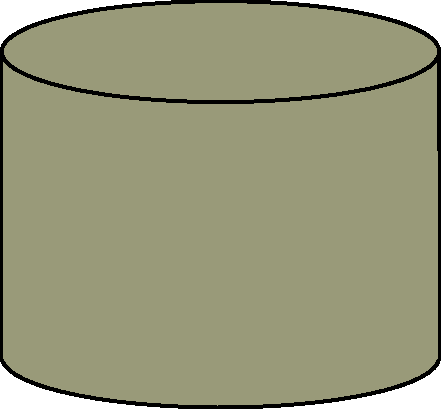
\includegraphics[width=5cm]{img/Konservendose.pdf}}
\end{center}

Der Hersteller, ein guter Freund von Ihnen, will exakt einen Liter
Zwiebelsuppe\footnote{S. \textit{Asterix} «Der goldene Kessel»} pro
Dose abfüllen.

Wie hoch, wie breit (Radius/Durchmesser) muss die Dose nun sein,
damit möglichst wenig Blech verwendet wird? Was sind Ihre
Überlegungen dazu?
